\documentclass[10pt,a4paper]{article}
\usepackage[utf8]{inputenc}
\usepackage[german]{babel}
\usepackage[T1]{fontenc}
\usepackage{amsmath}
\usepackage{amsfonts}
\usepackage{amssymb}
\usepackage{graphicx}
\author{Erik Zimmermann}
\begin{document}
\section{Druckoszillation zur Bestimmung von $\kappa$}
\begin{equation}
\text{Adiabatenindex: } \kappa= \frac{c_p}{c_V}=\frac{f+2}{f}
\end{equation}
mit $c_p$ Wärmekapazität bei konstantem Druck\newline
und $c_V$ Wärmekapazität bei konstantem Volumen\newline
für Luft ergibt sich mit
\begin{equation}
f=\underbrace{3}_{Translation}+\underbrace{2}_{Schwingung}=5 \Rightarrow \kappa=\frac{7}{5}=1,4
\end{equation} 
\begin{figure}[hbtp]
\caption{Rückhardt Methode}
\centering
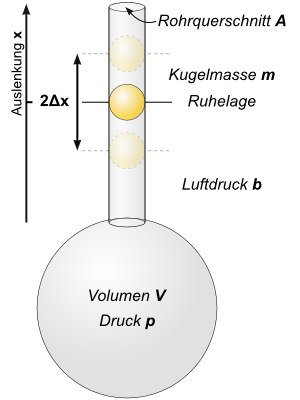
\includegraphics[scale=0.5]{4338.png}\end{figure}\\
wobei der Ball unter Lustdruck oszilliert, was eine Druckänderung hervorruft:
\begin{equation}
p=p_0+ \frac{m g}{A}
\end{equation}
mit der Rückstellkraft:
\begin{equation}
F=-\alpha \frac{dx}{dt}
\end{equation}
daraus ergibt sich die DGL:
\begin{equation}
m\frac{d^2x}{dt^2}=A dp - \alpha \frac{dx}{dt}
\end{equation}
da dieser Prozess adiabatisch ist folgt:
\begin{equation}
p V^{\kappa}=const \notag
\end{equation}
Differenzieren nach der Produktregel ergibt:
\begin{equation}
V^{\kappa} dp + p \kappa V^{\kappa -1} dV =0 \notag
\end{equation}
umstellen nach $dp$ und einsetzen von $dV=A x$ gibt:
\begin{equation}
dp=-\frac{p \kappa A x}{V}
\end{equation}
daraus folgt die DGL:
\begin{align}
\frac{d^2x}{dt^2}+\frac{\alpha}{m}\frac{dx}{dt}+ \frac{p \kappa A^2}{mV} x=0\\
\text{mit } \omega= \sqrt{\frac{p \kappa A^2}{mV}}\\
\Rightarrow \kappa = \omega^2\frac{m V}{p A^2}
\end{align}
\end{document}